\documentclass[a4paper,12pt]{article}
%\usepackage{fullpage}
%\usepackage{a4wide}
\usepackage[utf8]{inputenc}
\usepackage[danish, english]{babel}

% Nice looking font
%\usepackage{palatino}

% In order to highlight code
\usepackage[pdftex]{color}
\usepackage{listings}

% For graphics support
\usepackage{epsfig}
\usepackage{graphicx}
\usepackage{subfigure}

% Math support
\usepackage{amsmath}

% In order to include pdf
\usepackage{pdfpages}

% Graf support
%\usepackage{tkz-graph}

% Pdf section support
\usepackage{hyperref}
\hypersetup{
    bookmarks=true,         % show bookmarks bar?
    unicode=false,          % non-Latin characters in Acrobat's bookmarks
    pdftoolbar=false,       % show Acrobat's toolbar?
    pdfmenubar=false,       % show Acrobat's menu?
    pdffitwindow=true,      % page fit to window when opened
    pdftitle={OCamlCSP. A concurrency library for Ocaml}, % title
    pdfauthor={Joakim Ahnfelt-Rønne - 1986/03/14 - joakim.ahnfelt@gmail.com,
        Ramón Salvador Soto Mathiesen - 1979/05/15 - ramon@diku.dk and
        Advisor: Andrzej Filinski - andrzej@diku.dk}, % author
    pdfsubject={},   % subject of the document
    pdfnewwindow=true,      % links in new window
    pdfkeywords={keywords}, % list of keywords
    colorlinks=false,       % false: boxed links; true: colored links
    linkcolor=red,          % color of internal links
    citecolor=green,        % color of links to bibliography
    filecolor=magenta,      % color of file links
    urlcolor=cyan           % color of external links
}

% Macros
\newcommand{\missing}[1]{
  \begin{tabular}{|p{11cm}|}
    \hline
    \emph{Missing:} {\scriptsize (things that need to be written or considered)} \\
    \hline
    #1
    \hline
  \end{tabular}
}

\newcommand{\runtest}[1]{
  \footnotesize
  \framebox[14.5cm][l]{#1}
  \normalsize
}

\newcommand{\includecode}[2]{
  \definecolor{stringcolor}{rgb}{0.50,0.00,0.50}      %
  \definecolor{commentcolor}{rgb}{0.00,0.50,0.00}     %
  \definecolor{keywordcolor}{rgb}{0.00,0.00,1.00}     %
  \definecolor{idcolor}{rgb}{0.00,0.00,0.00}          %
  \lstset{language=ML,basicstyle=\ttfamily,keywordstyle=\color{keywordcolor},
    commentstyle={\color{commentcolor}\itshape},
    stringstyle={\color{stringcolor}},
    identifierstyle=\color{idcolor},numbers=left,
    xleftmargin=2em,% framerule=0.8pt,
    stepnumber=1,frame=tlrb,showstringspaces=false,
    firstnumber=1,numberstyle=\ttfamily, breaklines}

  \normalsize
  #1:
  \scriptsize
  \lstinputlisting{#2}
  \normalsize
}

\newcommand{\includeoutput}[2]{
\definecolor{allblackcolor}{rgb}{0.00,0.00,0.00}      %
\lstset{basicstyle=\ttfamily,keywordstyle=\color{allblackcolor},
        commentstyle={\color{allblackcolor}\itshape},
        stringstyle={\color{allblackcolor}},
        identifierstyle=\color{allblackcolor},numbers=left,
        xleftmargin=2em,% framerule=0.8pt,
        stepnumber=0,frame=tlrb,showstringspaces=false,
        firstnumber=1,numberstyle=\ttfamily, breaklines}

  \normalsize
  #1:
  \scriptsize
  \lstinputlisting{#2}
  \normalsize
}

% Opening
\title{OCamlCSP - a concurrency library for Ocaml}
\author{Joakim Ahnfelt-Rønne - 1986/03/14 - joakim.ahnfelt@gmail.com \and 
        Ramón Salvador Soto Mathiesen - 1979/05/15 - ramon@diku.dk \and
        \\ Advisor: Andrzej Filinski - andrzej@diku.dk}
\date{31$^{st}$ July 2009}

\begin{document}

\maketitle

\newpage
\selectlanguage{danish}
\begin{abstract}
% Grue: Højest 10 linjer: Hvad handler rapporten om? Hvilke resultater er
% opnået?
Her på dansk
\end{abstract}

\newpage
\selectlanguage{english}
\begin{abstract}
Here in english
\end{abstract}

\newpage
\tableofcontents
\newpage

% Line breaks between paragraphs instead of indentation
\parindent=0pt
\parskip=8pt plus 2pt minus 4pt

\section{Introduction}
This project is a complete, designed and implemented, API for a CSP-based
concurrency library in a functional language, in this case Ocaml\cite{?}.

We have achieved our three primary goals we set at the beginning:
\begin{itemize}
 \item \textbf{Designing an API for a CSP-based concurrency library in a
     functional language}. Because our main focus was on the API design, most of
   the {\it Section} \ref{analysis} is related to this.
 \item \textbf{Implementing the concurrency API in a functional language.} A
   complete description on how we implemendted the API based on the limitations
   of the chosen language?, use of a global lock. For more information look in
   the {\it Section} \ref{implementation}.
 \item \textbf{Assessing the API and underlying implementation by comparing
     applications built on top of it with similar applications built on top of
     an existing CSP library}. We have made a simple CSP network, Fibonacci,
   and a more complex, Webproxy, in order to test the API. The application are
   similar to the applications we have made for one of the other CSP libraries.
   A full description on how these applications are build and how to compile-run
   can be seen in the {\it Section} \ref{test}.
\end{itemize}

The resulting API source code and documentation can be seen in the Appendix
\ref{appendixSrc} and \ref{appendixDoc}. A online version is also avaliable at:

\begin{center}
http://github.com/Ahnfelt/mlcsp/
\end{center}

About the possible extensions to this API, we got wise on that we cannot
implement true parallelism through system threads, see at {\it Section
\ref{analysis}} for more information, but how we ``maybe'' can implement
parallelism with distribution through sockets, see {\it Section 
\ref{conclusion}}.

\section{Analysis}
\label{analysis}
\missing{
- Are CSP channels any2any and bidirectional? \\
- Are CSP channels names or values? \\
- Why don't we provide CSP events? \\
- References to CSP and CSP libraries. \\
- What do we do about shared state?\\
- Compare with the Event library.\\
- More introduction.\\
}

The CSP theory is concerned with processes that communicate solely by synchronous 
events. Synchronous channels are built on top of the basic abstraction, and this is
what most implementations (including \cite{occam}, \cite{c++csp}, \cite{jcsp} and 
\cite{pycsp}) provide for communication. 
Additionally, it is possible to wait for communication from multiple sources at once.

For each construct, we are going to look at how it's done in CSP and in the 
existing CSP libraries, how we would like to write it in OCaml, and what the 
semantics should be.

\subsection{Processes}
\missing{
- More about the lack of parallelism.\\
}

Processes can be run in parallel in CSP using the $\parallel$ operator:
\[P \parallel Q\]
The semantics of this is that the two processes $P$ and $Q$ are run in parallel. They
may communicate with each other. If put in front of another process in a sequence, all
processes running in parallel must finish before the next process can take any steps.

In PyCSP running two processes in parallel looks like this:
\begin{verbatim}
Parallel(P, Q)
\end{verbatim}
Where $P$ and $Q$ must be specified as $Process$ instances. It runs the processes in
parallel and returns when they have all stopped executing. Since Python does not offer
a literal syntax for such objects that can be used in a expression, the processes must
be defined elsewhere. The API for C++CSP and JCSP are similar, although Java does offer
object literals. In all cases the object literals only expose a \emph{run} method. 
It is unclear what happens if this method is called twice on the same instance 
(especially if the instance is used twice in the same parallel-construct).

To avoid undefined behaviour we use functions to represent process definitions. There is 
nothing special about the functions except that they have the type $unit \to unit$. OCaml 
allows us to treat the functions as values, which means we can pass them around and use 
them as arguments for our parallel construct:

\begin{verbatim}
parallel [P; Q]
\end{verbatim}

However, since OCaml has anonymous functions, we can define the process directly inside
the parallel construct, which is often convenient for small processes. The processes
are then run in parallel, and there is no way to get a handle to a \emph{running} process
through our API.

Sometimes it is useful to define a function that starts a process as a side effect, but
returns before the process has finished. This corresponds to running the process in 
parallel with \emph{the rest of the program}. Since we don't have continuations, we 
provide the special purpose function \emph{fork} that simply starts a process and returns
immediatly. JCSP does something similar with their \emph{ProcessManager}, but provides a
\emph{stop} method that will terminate the process. It has since been deprecated because
it is unsafe to terminate a running process from the outside. There is not much else to 
do with a handle to a process, so we avoid returning a handle to it at all.

We don't provide a special construct for sequence, since OCaml has a perfectly fine 
sequence operatoer built in, and executing a list of processes in sequence is a simple
matter of iterating over it and invoking each one. We also don't provide a way to specify 
the stack size for a process, because the stack grows dynamically in OCaml user threads, 
and there is little reason to use system threads (see section \ref{implementation}).

Note that the library \emph{does not provide parallel execution}; it only provides 
perceived concurrency (see section \ref{implementation}).

\subsection{Channels}
\missing{
- Why don't we have broadcasts or any2all?\\
}

Channels are the only means of communication between processes that we provide directly.
In PyCSP, C++CSP and JCSP, channels are created by constructing an instance of a channel
class. Our channels correspond to their \emph{any2any} channels, meaning that any number
of processes can send on and receive from a channel, that any message sent over it
has exactly one sender and one receiver, and that these communicate synchronously.

Creating a channel is just a call to a function which returns the new channel:
\begin{verbatim}
let c = channel ()
\end{verbatim}

Two of the basic constructs for CSP channels are send and receive:
\[c\,!\,e \to P\]
\[c\,?\,x \to Q(x)\]
Where $c$ is a channel, $e$ is an expression, $x$ is a name and $P$ and $Q$ are processes. 
The semantics of these are to synchronously send or receive a value respectively, and
then become another process. In the case of receive, the process may refer to the
received value $x$.

In PyCSP, these two constructs look like this:
\begin{verbatim}
c.write(e)
P
\end{verbatim}
\begin{verbatim}
x = c.read()
Q(x)
\end{verbatim}
It's using methods to realize the read/write, and sequence to realize \emph{becoming}
another process after the synchronization. Note that the channels are values, whereas
they are names in CSP. JCSP and C++CSP are similar.

The obvious way to look like CSP is to define operators ! and ? that works like the
CSP counterpart. However, it is not possible in OCaml to declare that the right hand 
side of the question mark introduces a binding. It is also not desireable to redefine
the ! operator that is used for dereferencing mutable references in OCaml.

We therefore have to decide between methods and functions. The OCaml standard library
primarily uses functions to provide it's functionality, and few if any other ML 
variants share OCaml's object model. Since we don't anticipate any need for an
exstensible inheritance hierachy for channels, we choose functions for the task.
We use the \textbf{let in} construct to provide binding.

\begin{verbatim}
write c e; P
\end{verbatim}
\begin{verbatim}
let x = read c in Q(x)
\end{verbatim}

It is possible to transmit any OCaml value over a channel, including impure functions and mutable 
state. Sharing mutable state between processes should only be done with caution however, since it 
requires additional synchronization beyond the scope of this library. The remaining semantic 
details of the channels are explained in the following section.

\subsection{Alternation}
\missing{
- PriSelect (not there because it's not well defined).\\
- FairSelect (what problem does this actually solve?).\\
- Polling or skip guards (can be implemented as a process). \\
- Time guards (can be implemented as a process). \\
}

Alternation corresponds to \emph{external choice} in CSP, which uses the $|$ operator:
\[c_1\,?\,x \to P(x)\ |\ c_2\,?\,x \to Q(y)\ |\ c_3\,!\,e \to R\]
The semantics is that once one or more of the alternatives can take a step, then
an arbitrary one of these is chosen to take a step, and then the whole process acts as 
the remainder of the chosen alternative.

In PyCSP it looks like (where in1 = c1.read, in2 = c2.read, out3 = c3.write):
\begin{verbatim}
s = Alternative(in1, in2, out3).priSelect()
if s == in1:
    x = in1()
    P(x)
elif s == in2:
    y = in2()
    Q(y)
else:
    out3(e)
    R
\end{verbatim}

Note that the whole if-construct can be replaced by an application if all the guards have the same type 
and become the same process. The JCSP and C++CSP selects take in a list of guards and return the index
of the guard, which you can then switch on. In both cases, you have to \emph{promise} to read from the
chosen channel, or the behaviour will be undefined.

Starting from CSP's syntax, we might want to write something like \texttt{(A | B | C)}, where $A$, $B$
and $C$ are processes. If we consider process definitions functions of type $unit \to unit$ for this 
purpose, one might define an operator $|$ that takes two processes and returns the result of the one that 
is chosen. The problem with this is that it is very hard in plain OCaml to inspect functions at runtime 
to see which one of them can take a step.

Instead we make the first step inspectable by providing \emph{guards}, which is also the route taken by
the other libraries. However, we would like to avoid relying promises and idioms to obtain the 
intended behaviour. We therefore make the action an integral part of each guard. We use a list instead
of an operator in order to provide a more natural syntax for alternation with more than two choices.

\begin{verbatim}
select [
    read_guard c1 P(x);
    read_guard c2 Q(y);
    write_guard c3 e R;
]
\end{verbatim}
Where $P(x)$ and $Q(x)$ are functions that take the read value as a parameter, and $R$ takes the written 
value. Anonymous functions can be used to give it the appearence of a control construct. Note that select 
also returns the result of the chosen action, which is particularily convenient if you are reading and 
don't care which channel the value comes from.

In CSP, any process that can take a step may be chosen arbitrarily. However, if the same list of 
alternatives is used in a loop, this might lead to starvation. If one of the guards is always ready,
an arbitrary choice can be to chose this one every time. This means that any other guards that are 
ready will be skipped indefinatly, and thus be starved.

We solve this by prioritizing the guards in a random order each time select is called. That way the
chance that a ready guard is not taken approaches zero as the number of calls to select grows. Note 
that this is also a valid behaviour of the arbitrary choice, which we don't provide separatly.

The \emph{read} and \emph{write} functions are semantically equivalent to a select that has exactly 
one guard.

The semantics of the select so far is to block until one of the guards become ready. The obvious
way to define a select with no guards at all is therefore to block indefinatly, causing a deadlock.
Preferably, the thread would not take up any further resources in this case (since it's trivial to 
detect), and thus we attempt to terminate the thread by throwing an exception. If stack traces are
enabled, and the empty select is an error, this might also provide the programmer with more information
to determine where the error occured.

We do not provide any API for internal choice, since OCaml has plenty of control structures built-in.
In JCSP and C++CSP you can provide a list of flags that specify if a guard is active or inactive. We
do not provide this as it is just as easy to simply filter the list of guards.

\subsection{Termination of process networks}
\missing{
- What happens if some but not all alternatives in a select is poisoned? \\
- Automatic poison propagation (PyCSP has it by relflection)\\
- Read up on CSP interrupts and see if they could provide safe termination and propagation.\\
}

Since no practical applications run forever, safe termination of process networks should be considered.
One way to implement this is to send a special termination message. However, that requires insertion of 
termination logic for every communication where the process might receive a termination message.
Additionally, if the reader wants to terminate the writer, it might require a dedicated channel 
just for termination messages.

\subsection{Permissions}
\missing{
- Permissions.\\
- Purely implemented in the type system.\\
}

\section{Implementation}
\label{implementation}


\subsection{Channels}
A one to one channel is a channel that only allows one procees to read from it and one process 
to write to it. It may be implemented as a state machine as shown in figure \ref{channel-state}.
When the channel is in the NobodyWaiting state and a process tries to read from the channel,
it enters the ReaderWaiting state. When a writer comes along and tries to write to a channel
in this state, it returns to the NobodyWaiting state, transfers the message, and only then
allows the two processes to continue. The WriterWaiting state works in much the same way.

\begin{figure}[h]
\centering
\includegraphics[width=0.6\textwidth]{channel-state.png}
\caption{Simplified channel state (poison and multi-read/write not shown)}
\label{channel-state}
\end{figure}

From any state, the channel might be poisoned and enter the Poisoned state. If it was in the
ReaderWaiting or the WriterWaiting state, the waiting process will wake up and throw a special
exception. Any further attempts to read from or write to the channel will result in this 
exception being thrown again.

For any to any channels that places no restrictions on the number of processes that can read
from or write to it, we simply extend the above to keep a queue of readers (when in the 
ReaderWaiting state) or writers (when in the WriterWaiting state).

The choice of using a queue gives a stronger guarentee than CSP gives, namely that no processes
will be starved. By starvation we mean to say that a process waiting to read or write on the
channel can be blocked indefinately even though an infinite number of messages is transmitted
over the channel. This would happen with a stack if another process is always ready to read or 
write again before the channel was ready to accomodate the starving process. The starving process
would always be put behind the eager process with a stack, but with a queue, the starving process
will always advance in the queue every time a message is transmitted, guarenteeing that it will
eventually get it's turn.

In order to only wake up the waiting process, each process has it's own condition variable that
it waits on. Additionally, readers have a function that takes in a value and performs a side 
effect, while writers have a function that performs a side effect and produces a value. The side
effect for both is to set it's internal reference to the transmitted value (instead of None),
remove it from all the channels it's listening on and wake up the process.

We use a lock that is global to the library, in order to protect the channel and processes from
concurrent mutation. This lock is only ever taken when first trying to read from a channel, or
right after a process has been woken up. We claim that this won't lead to performance degradation,
since OCaml's threads only provides concurrency though time-sharing \cite{ocaml-threads}.

\missing{
- How do you get rid of this lock? (useful for porting). It is hard because you don't know which
channels you will touch before you have chosen a target process to transmit to/from. If you knew
that, you could simply take their locks in some well defined order (thus avoiding deadlock). \\
}

\begin{verbatim}
type 'a channel_state
    = NobodyWaiting 
    | ReaderWaiting of (Condition.t * ('a -> unit)) list
    | WriterWaiting of (Condition.t * (unit -> 'a)) list
    | Poisoned

type ('a, 'b) channel = ('a channel_state) ref
\end{verbatim}

The phantom type 'b is used for the channel permissions. This is enforced solely via the type
system, and is represented with a product of three booleans values: read * write * poison.
Reading, writing and poisoning are initially enabled for a channel, but handles with less 
permissions can be obtained through the functions shown in figure \ref{channel-permissions}. 
Permissions can only be taken away, not gained, which is evident from the types of the 
functions, for example: 

\begin{verbatim}
val read_poison_only : ('a, on * _ * on) channel -> 
                       ('a, on * off * on) channel
\end{verbatim}

Apart from the type, all of these functions are simply identity functions. We provide a
type alias \texttt{'a t = ('a, on * on * on) channel} for people who don't want to write the
longer (often optional) type annotations that the permission types incur.

\begin{figure}[h]
\centering
\begin{tabular}{c|c|c|l}
Read & Write & Poison & Function \\
\hline
0 & 0 & 0 & (useless) \\
0 & 0 & 1 & poison\_only \\
0 & 1 & 0 & write\_only \\
0 & 1 & 1 & write\_poison\_only \\
1 & 0 & 0 & read\_only \\
1 & 0 & 1 & read\_poison\_only \\
1 & 1 & 0 & read\_write\_only \\
1 & 1 & 1 & (default) \\
\end{tabular}
\caption{Channel permissions}
\label{channel-permissions}
\end{figure}

\subsection{Alternation}

\missing{
- Occam does not seem to sufficiently describe PRI ALT when two processes with inverse priorities
on the same two channels use it (in the manual). This is why we don't support it. \\
- Consider supporting something a bit like PRI ALT anyway since it's easier to build on top of
than the current randomized select. \\
}

\subsection{Processes}

\section{Test}
\label{test}
One of the goals for this project was that we needed to implement a simple
network on top of the API, Fibonacci, and a more complex network, The Ising 2D
Model.

Because Ocaml doesn't have support for parallelism, as mentioned in the Analysis
Section\ref{?}, we decided to make a Webproxy, with a build in cache.

But before we made this two applications we needed to now the limitations of
Ocamls Thread library and IO Library.

A detailed description on how to run the test can be seen in
Appendix \ref{appendixTest}.

\subsection{Performance}

%\begin{table}[ht]
%\centering
\begin{tabular}{|p{3cm}|p{8.5cm}|c|}
    \hline
    	File name &
	Description &
	Result \\
    \hline
    	maxthreads.ml (user thread) &
        The application creates as many threads as possible, once it reaches
        about 15.000 it stops spawning more threads (deadlock ?).&
	FAIL \\
    \hline
    	maxthreads.ml (system thread) &
        The application creates as many threads as possible, once it reaches
        about 100 it stops spawning more threads (deadlock ?).&
	FAIL \\
    \hline
    	nonblocking.ml &
        We run to processes in parallel. The first process whats for user input
        and the second process after a seconds delay reads the first line from
        the its own source code file and writes the line to stdout.&
	OK \\
    \hline
    	commstime.ml &
        A benchmark application used by Brian Vinter to measure PyCSP vs JCSP.&
	OK \\
    \hline
  \end{tabular} 
%\caption{The first three test checks Ocaml implementation of the Thread library
%  and I/O. In the last test, we compare OcamlCSP vs PyCSP.}
%\label{testtable}
%\end{table}

\subsubsection*{Maxthreads}
In this test we try to find an upperbound of how many threads we can create,
user threads or system threads. In the first case when using user threads we
find that after creating between 15.000 - 20.000 threads the application
freezes. We are not able to find any kind of documentation that can helps us
verify that it's a deadlock or a maximum number of threads allowed for an
application to create. If we run the test several times, we will see that
each application will be able to create about those 15.000 - 20.000 threads.

In case it's a limitation in Ocaml, we could by implementing sockets always
start $n$ times the application and make them comunicate over sockets so we
could achieve the number of threads as we desire.

In the second test based on maxthreads, we use system threads and as before
the application freezes but just after creating about 100 threads.


\subsubsection*{Nonblocking}
To implement the Webproxy we need to know if one of the processes is waiting
to recieve a chunck of data, if it block the IO until it has recieved the data
or if another process that is also waiting for a chunck.

We discovered that Ocaml support non-blocking IO so it will be no problem have
several clients waiting to recieve data from our Webproxy. An example could
be a client that connects over the Webproxy to a very slow website. The website
can only deliver a small amount of data every second. If another client that
also connects over the Webproxy to a fast website. While the first client
waits to recieve data from the webserver, the second client can read chunks
of data from the fast website.


\subsubsection*{Commstime}
Even though we don't set focus on performance and optimization, we still wanted
to implement the Commstime\cite{vinterpycsp} process that's used to compare
PyCSP against JCSP.

The only change we made to the code is that we use {\it Unix.gettimeofday} in
order to get the same time precision as Pythons {\it time.time} has. By running
both application on the same computer\footnote{Macbook Pro 2,6 GHz Core 2 Duo
4GB RAM. Mac OS 10.5.7}, we achieve a execution time that it's about twenty
times faster.


\subsection{Fibonacci}

TODO: A picture of network (made with tkiz) goes here !!!

... under test running fibonacci we discovered that our components weren't tail
recursive so we get a Stack overflow when we reached the 75.000 iteration. We
solve it by using while true ...

\subsection{Webproxy}

TODO: A picture of network (made with tkiz) goes here !!!

\section{Conclusion}
\label{conclusion}

If we compare how Brian Vinter teaches CSP\cite{vintercsp}:
\begin{center}
\begin{verbatim}
PairsInt (in, out) = Delta2Int (in, a, c) || 
                     TailInt (a, b) || 
                     PlusInt (b, c, out) 
\end{verbatim}
\end{center}

versus how we implement the simple network:

\begin{verbatim}
let pairsInt i o () =
  let a = Csp.channel () in
  let b = Csp.channel () in
  let c = Csp.channel () in
    Csp.parallel [
      delta2int i a c;
      tailint a b;
      plusint b c o;
    ]
\end{verbatim}

We can see that there is almost no difference beside the {\it parallel operator}
and definition of the channel variables.

% ----------------------------------------------------------------------
% Bibliography
% ----------------------------------------------------------------------
\newpage
\begin{thebibliography}{99}

\bibitem[Hoare 04]{hoare}
:\\
Communicating Sequential Processes\\
C. A. R. Hoare\\
Prentice Hall International; (June 24, 2004)\\
ISBN-10: 0-13-153271-5\\
ISBN-13: 978-0-13-153271-7\\
http://www.usingcsp.com/cspbook.pdf


\bibitem[Vinter, PyCSP]{vinterpycsp}
:\\
PyCSP. The beginning of a CSP library for Python\\
Brian Vinter\\
Department of Computer Science. University of Copenhagen\\
http://isis.ku.dk/kurser/blob.aspx?feltid=224718\\
Last visited: $20^{th}$ july 2009

\bibitem[Vinter, CSP]{vintercsp}
:\\
Threading\\
Brian Vinter\\
Department of Computer Science. University of Copenhagen\\
http://isis.ku.dk/kurser/blob.aspx?feltid=224185\\
Last visited: $20^{th}$ july 2009



\end{thebibliography}
% ----------------------------------------------------------------------

\appendix
\newpage
\section{Appendix: Source code}
\label{appendixSrc}

\scriptsize
\subsection{API}
\label{appendixAPI}
\includecode{csp.mli}{../source/csp.mli}
\includecode{csp.ml}{../source/csp.ml}
\subsection{A CSP Utility Library}
\includecode{cspu.ml}{../source/cspu.ml}
\subsection{A CSP Component Library (Legoland)}
\includecode{legoland.ml}{../source/legoland.ml}


\newpage
\section{Appendix: Documentation}
\label{appendixDoc}
\begin{center}
  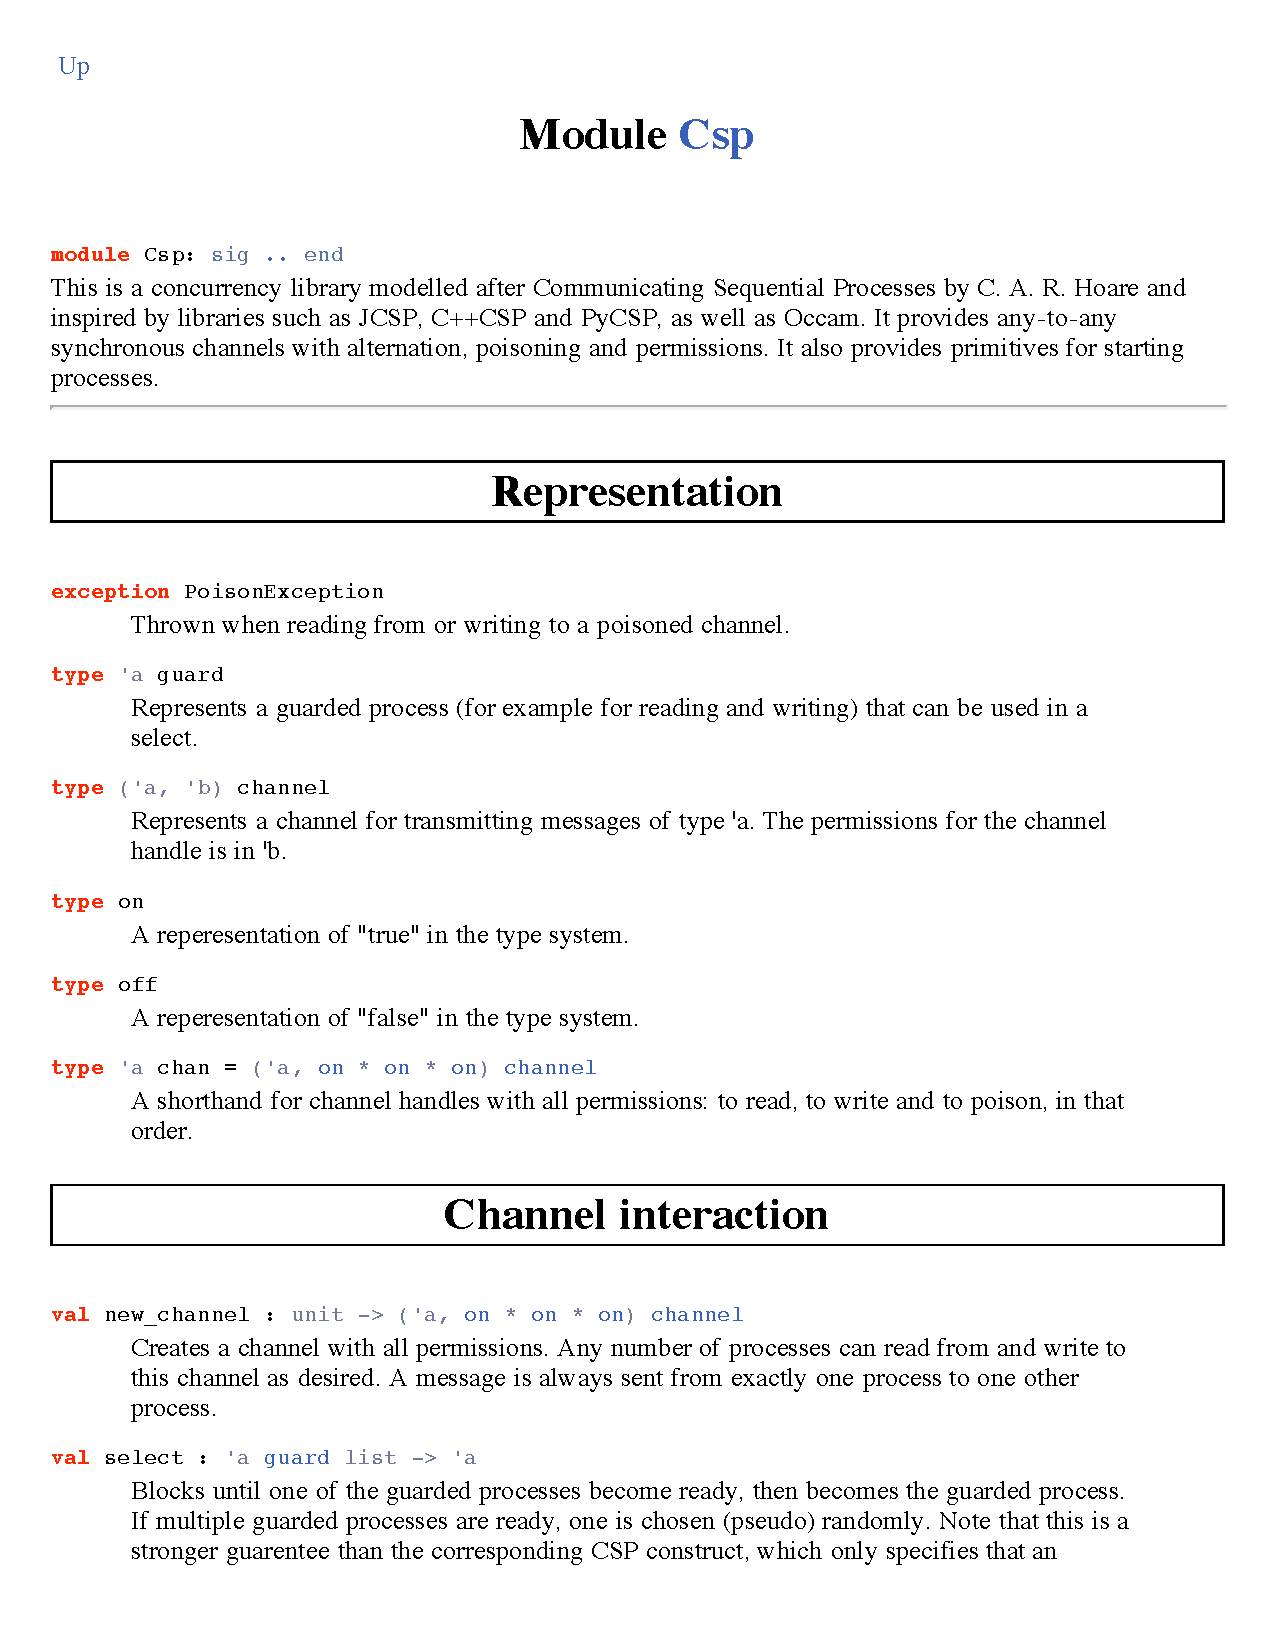
\includepdf[pages=-]{../docs/csp.pdf}
\end{center}


\newpage
\section{Appendix: Test}
\label{appendixTest}
\subsection{Performance}

\subsubsection{Maxthreads}
\includecode{maxthreads.ml}{../test/maxthreads.ml}
\runtest{ocamlc -vmthread unix.cma threads.cma maxthreads.ml -o maxthreads \&\&
  ./maxthreads}
\includeoutput{userMaxThreads.txt}{test/userMaxThreads.txt}
\runtest{ocamlc -thread unix.cma threads.cma maxthreads.ml -o maxthreads \&\&
  ./maxthreads}
\includeoutput{sysMaxThreads.txt}{test/sysMaxThreads.txt}

\newpage
\subsubsection{Nonblocking}
\includecode{nonblocking.ml}{../test/nonblocking.ml}
\runtest{ocamlc -vmthread threads.cma unix.cma nonblocking.ml -o nonblocking
  \&\& ./nonblocking}
\includeoutput{nonblocking.txt}{test/nonblocking.txt}

\subsubsection{Commstime}
\includecode{commstime.ml}{../test/commstime.ml}
\runtest{./buildCommstime.sh \&\& ./commstime}
\includeoutput{ocamlcsp\_commstime.txt}{test/ocamlcsp_commstime.txt}
\includeoutput{pycsp\_commstime.txt}{test/pycsp_commstime.txt}

\subsection{Fibonacci}
\includecode{fibCSP.ml}{../test/fibCSP.ml}
\runtest{./buildFibCSP.sh \&\& ./buildFibCSP}
\newpage
\includeoutput{fibonacci.txt}{test/fibonacci.txt}

\newpage
\subsection{Webproxy}
\includecode{proxyCSP.ml}{../test/proxyCSP.ml}
\includecode{server.rb}{../test/web/server.rb}
Start two sequential webservers (ruby):

\runtest{ruby server.rb 4040 0.1 \&}

\runtest{ruby server.rb 4041 0.3 \&}


Start the webproxy:

\runtest{./buildProxy.sh \&\& ./proxyCSP \&}


Add the webproxy to the terminal session:

\runtest{export http\_proxy=http://localhost:8080}


Retrieve the file foo.mp3 from the first webserver:

\runtest{wget http://localhost:4040/foo.mp3}
\includeoutput{proxy\_get\_file\_first\_time.txt}{
  test/proxy_get_file_first_time.txt}


Retrieve the file foo.mp3 again from the first webserver (cache):

\runtest{wget http://localhost:4040/foo.mp3}

\includeoutput{proxy\_get\_file\_second\_time.txt}{
  test/proxy_get_file_second_time.txt}


Retrieve concurrent the files bar.mp3 and foo.mp3 from the two webservers:

\includeoutput{proxy\_same\_time\_bar.txt}{
  test/proxy_same_time_bar.txt}
\includeoutput{proxy\_same\_time\_foo.txt}{
  test/proxy_same_time_foo.txt}


\end{document}
